% This is samplepaper.tex, a sample chapter demonstrating the
% LLNCS macro package for Springer Computer Science proceedings;
% Version 2.20 of 2017/10/04
%
\documentclass[runningheads]{llncs}

\usepackage{graphicx}
\usepackage{subcaption}
\usepackage{xcolor}
\usepackage{tikz}
\usepackage{bm}
\captionsetup{compatibility=false}
\captionsetup[figure]{labelfont={bf}}
\captionsetup[table]{labelfont={bf}}
\captionsetup{labelsep= period}



% Used for displaying a sample figure. If possible, figure files should
% be included in EPS format.
%
% If you use the hyperref package, please uncomment the following line
% to display URLs in blue roman font according to Springer's eBook style:
% \renewcommand\UrlFont{\color{blue}\rmfamily}

\begin{document}
%

\title{The Investigation of Citation On Google Scholar, Web of Science and Scopus }
%
%\titlerunning{Abbreviated paper title}
% If the paper title is too long for the running head, you can set
% an abbreviated paper title here
%
\author{Xiankun Yan\inst{1}}
%
\authorrunning{Y. Xiankun}
% First names are abbreviated in the running head.
% If there are more than two authors, 'et al.' is used.
%
\institute{University of Birmingham, Birmingham B15 2TT, UK }
\titlerunning{The Investigation of Citation On Three Different Services }
\maketitle
%

%
\begin{abstract}
Nowadays, the citation is a significant method to assess the quality of the paper. In different academic services, they provide different results about the retrieved citation. In this paper, based on three factors including currency, the proportion of each type of citation, and use efficiency, Google Scholar, Web of Science and Scopus are analyzed to evaluate the quality of each service. Finally, Google Scholar has a strong ability to get lots of different kinds of recent citations, but it is hard to use. Compared to the Google Scholar, Web of Science cannot get too many recent quotations and the retrieved result's types gather in two sorts,  this system, however, is easy to use. The performance of Scopus is similar to Web of Science, but this service has access to retrieve more recent citations than Web of Science.

\keywords{Citation  \and Google Scholar \and Web of Science \and Scopus.}
\end{abstract}
%
%
%
\section{Introduction}
\subsection{Background }
Nowadays, the citation becomes an important way to evaluate the quality of one paper. In 1985, Sharplin and Mabry indicated the most common method to rank the quality of one publication is the citation. And they also said the purpose of the journal is to teach knowledge about this major. Therefore, the number of quotation reflects the quality of the researcher's journal~\cite{sharplin1985relative}. And in 1996, Robert J. said some studies have shown a net number of citations after subtracting 'self-citation' which are journal citations from the same journal. This is aim to decrease any possible bias in the article selection process~\cite{vokurka1996relative}.
\par\noindent
\\
Many academic services provide access to observe quotation like Google Scholar, Web Of Science, Scopus and so on. However, due to the difference of search algorithms, the results would be different when users search the relevant citations. In 2008, Alireza Noruzi found Google Scholar provides a free alternative or complement to other citation indexes~\cite{harzing2008google}. However, in 2010, Miguel A. and Garc{\'\i}a-P{\'e}rez think the citations retrieved by Web of Science had the high related rate to the seed paper~\cite{garcia2010accuracy}. And Lokman I. , Meho and Kiduk Yang believe Scopus also has the ability to get a comprehensive picture of the scholarly impact of authors in 2007~\cite{meho2007impact}. Therefore, how to choose the best services is also a question that deserves to be considered carefully.

\subsection{Related Work}
In the paper, in order to investigate the quality of different academic service, five papers (see in the Table~\ref{tab:my_label}) from Philip S. Yu who work in the University of Illinois at Chicago are selected as the seed papers. And three service (Google Scholar, Web of Science and Scopus) are used to search the 10 recent papers citing each seed papers. 
\par\noindent\\
Besides, four questions contribute to analyzing the result:
\begin{enumerate}
    \item Are there significant differences in the citations retrieved by each of these services?
    \item How well does each service provide access to the core forms of the literature of Computer Science?        
    \item What is the currency of each the service?
    \item Subjectively, how easy is each of the systems to use?
\end{enumerate}
In terms of data analysis and four questions, this paper would use some statistics knowledge to assess the quality of each service from three factors: the currency, the proportion of each type of citation and use efficiency.
\par\noindent\\
Besides, this paper uses the style about the Springer's Lecture Notes in Computer Science\footnote{About Further information, please check in  https://www.springer.com/gp/computer-science/lncs/conference-proceedings-guidelines.}.
\begin{table}[ht]
    \setlength{\abovecaptionskip}{10pt}%    
    \setlength{\belowcaptionskip}{0pt}%
    \caption{The five seed papers from Philip S. Yu}
    \centering
    \begin{tabular}{|c|p{0.7\columnwidth}|c|}
    \hline
        No. & paper's name & year of publication  \\
    \hline
         1. & A general framework for relation graph clustering & 2010 \\
   
         2. & Equivalent thickness conception for corner cracks & 2010\\
    
         3. & On clustering massive text and categorical data streams & 2010\\
    
         4. & Statistical downscaling of daily precipitation using support vector machines and multivariate analysis & 2010\\
   
         5. & Comparison of genetic algorithms and shuffled complex evolution approach for calibrating distributed rainfall-runoff model & 2010 \\ 
    \hline
    \end{tabular}
    
    \label{tab:my_label}
\end{table}

\section{The Processing Of Investigation  }
\subsection{Data collection and visualization}
In this paper, the five seed journals in 2010 are selected from Philip S. Yu. Then, three websites are used to search papers that cite the seed paper. About 71 quotations are retrieved by three academic web service. In this paper, in order to clearly show all data, the Venn diagram~\cite{freiler2008interactive} are used to present the distribution of data on different services(See in Fig.~\ref{fig1}).
%draw Venn diagram
\begin{figure}
\centering
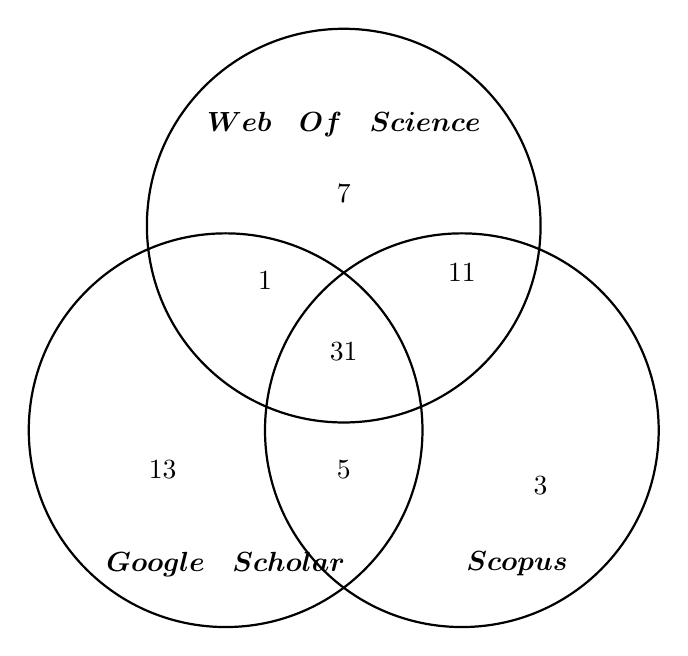
\begin{tikzpicture}[thick]
        \draw (0,0) circle (2.5) node[above,shift={(0,-2)}] {$\bm{Google\quad Scholar}$};
        \draw (60:3cm) circle (2.5) node[above,shift={(0,1)}] {$\bm{Web\quad Of\quad Science}$};
        \draw (0:3cm) circle (2.5) node[shift={(0.7,-1.7)}] {$\bm{Scopus}$};

        \node at (1.5,1) {31};
        \node at (0.5,1.9) {1};
        \node at (4,-.7) {3};
        \node at (1.5,-.5) {5};
        \node at (3,2) {11};
        \node at (-.8,-0.5) {13};
        \node at (1.5,3) {7};
\end{tikzpicture}
\caption{The distribution of different citations on three service} \label{fig1}
\end{figure}
\par
\noindent
\\
From the distribution of those data,  31 same journals can be found on those websites. And also the maximum part of the same papers are included in the Web of Science and Scopus about 42 papers. For the second large overlap section, it is about 36 papers in the Google Scholar and Scopus, which is less than the maximum one about 6 papers. In addition, remaining parts that do not have any overlap section respectively are 13 papers in Google Scholar, 7 Papers in Web of Science and 3 papers in Scopus.
\par\noindent\\
Therefore, depending on this distribution figure, it shows the abilities of those three services to find citation are different. 

\subsection{Data analysis}
In this paper, three factors that respectively are the currency, the proportion of each type of citation and use efficiency would be used to evaluate the capacity of three academic services.
\subsubsection{Currency}
\par\noindent\\
When lots of citations are retrieved by three websites, they are sorted by time and got accounted in Table~\ref{tab:my_label2}. Relay on the year of publication, the ability of each service to retrieve recent quotations could be shown. Services that have strong ability to search recent citations would have a higher occupation in 2018 and a lower proportion in other years.
\begin{table}
    \setlength{\abovecaptionskip}{10pt}%    
    \setlength{\belowcaptionskip}{0pt}%
    \caption{The number of papers in different year (2011-2018)}
    \centering
    \begin{tabular}{|c|c|c|c|c|c|c|c|c|}
    \hline
        Service's name & In 2018 & In 2017& In 2016& In 2015& In 2014& In 2013& In 2012& In 2011  \\
    \hline
         Google Scholar & 29 & 4 & 10 & 2 & 3 & 2 & 0 & 0 \\
    
         Web of Science & 16 & 8 & 14 & 1 & 3 & 4 & 3 & 1\\
    
         Scopus  & 22 & 8 & 9 & 2 & 4 & 4 & 1 & 0\\
    \hline
    \end{tabular}
    
    \label{tab:my_label2}
\end{table}
\par\noindent
According to the Table~\ref{tab:my_label2}, It can be found vividly that the Google Scholar find the maximum number of papers about 29 papers comparing to 22 papers in Scopus and 16 papers in Web of Science respectively. Besides, only one paper can be retrieved by the Web of Science, but the Google Scholar and Scopus could not get anyone. For the remaining papers from 2012 to 2017, they are approximately 66\%, 56\% and42\% of the total in Web of Science, Scopus and Google Scholar respectively. Hence, from those statistics, it reflects that the Google Scholar has the most strong capacity of getting the new citations than the Scopus and the Web of Science.

\subsubsection{The proportion of each type of citation }
\par\noindent\\
In this paper, the proportion of each type of citation also is an important factor to evaluate the performance of each service. There are about 3 types including article, conference and others and all the ratios are accounted in Fig.~\ref{fig2}.

\begin{figure}[ht]

\begin{subfigure}{0.5\textwidth}
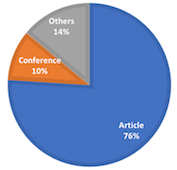
\includegraphics[width=0.9\linewidth, height=5cm]{Picture1.png}
\caption{Google Scholar}
\label{fig:subim1}
\end{subfigure}
\begin{subfigure}{0.5\textwidth}
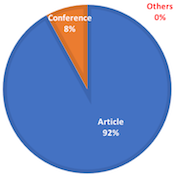
\includegraphics[width=0.9\linewidth, height=5cm]{Picture2.png}
\caption{Web of Science}
\label{fig:subim2}
\end{subfigure}
\begin{subfigure}{0.5\textwidth}

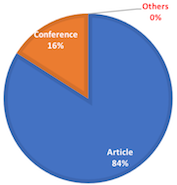
\includegraphics[width=0.9\linewidth, height=5cm]{Picture3.png}
\caption{Scopus}
\label{fig:subim3}
\end{subfigure}
\captionsetup{labelsep = period}
\caption{The proportion of each kind of citations in different websites}
\label{fig2}
\end{figure}
\par
\noindent\\
From three pies, the common phenomenon is the parts of the Article are the maximum proportion in all service. In terms of the Web of Science, the proportion of Article occupies about 92\%, which is more than 10 times as large as the Conference. Similarly, There is 84\% about Article in the Scopus, which also is more than 5 larger than the others. And the Others types of quotation are 0\% in the Web of Science and the Scopus. However, it is different in the Google Scholar, where the percentage of Others is 14\% and is higher than Conference about 4\%. As for the ratio of Article in the Google Scholar, it accounts for 76\%, which also is the main part.
\par\noindent\\
Though the analysis of each pie, Web of Science can get the most citations about the Article type. However, Google Scholar provides access to find lots of kinds of citations.
\\


\subsubsection{Use Efficiency}
\par\noindent\\
In this paper, the steps used to get the recent citations of each seed papers would be counted to evaluate the use efficiency and the statistical data would be shown in the below table~\ref{tab:my_label3}.

\begin{table}
    \setlength{\abovecaptionskip}{10pt}%    
    \setlength{\belowcaptionskip}{0pt}%
    \captionsetup{labelsep= period}
    \caption{The steps used to get recent citations of each seed paper }
    \centering
    \begin{tabular}{|c|c|c|c|}
    \hline
         &Google Scholar& Web of Science& Scopus  \\
    \hline
         The number of steps & 5 & 2 & 2 \\
    \hline
    \end{tabular}
    \label{tab:my_label3}
\end{table}
\par
\noindent
From table~\ref{tab:my_label3}, Google Scholar is more complex to get the new quotations than the others, which need 5 steps. Both Web of Science and Scopus only need 2 steps to retrieve relevant citations. Therefore, Web of Science and  Scopus are easier to use than Google Scholar.


\subsection{Conclusion}
From three factors including currency, the proportion of each type of citation and use efficient, the performances of each service are analyzed and shown in the table~\ref{tab:my_label4}.
\begin{table}[ht]
    \setlength{\abovecaptionskip}{10pt}%    
    \setlength{\belowcaptionskip}{0pt}%
    \caption{The performances of each service }
    \label{tab:my_label4}
    \centering
    \begin{tabular}{|l|l|l|l|}
    \hline
         &Google Scholar& Web of Science& Scopus  \\
    \hline
         The kinds of citations & multiple & not many & not many \\
    
         Currency & lots of new citations & little of new citations & most of  new citations \\
    
         Use efficient  & difficult & easy & easy \\
         
    \hline
    \end{tabular}

\end{table}
\par\noindent
From that analysis, three services differ on their performance. The Google Scholar can retrieve kinds of recent citations compared to the others. However, the Scopus is easy to use and also can get most of the recent quotations. In terms of Web of Science, it is similar with the Scopus but the retrieved citations gather at two types.


\section{Summary}

In this paper, the differences about the quality of retrieval result between Google Scholar, Web of Science and Scopus are investigated based on three factors including currency, the proportion of each kind of quotation and use efficiency. According to the performance of each academic service, Google Scholar has a strong ability to get lots of new quotations that belong to lots of different types, but it would be not easy to use compared to the others. The most of the citations retrieved by the Web of Science published in the old year and do not have many kinds, but use efficiency of this service is higher than Google Scholar. In terms of Scopus, this system is easy to use and can get most of the recent quotations, but the citations retrieved by it also only about two sorts.



%
% ---- Bibliography ----
%
% BibTeX users should specify bibliography style 'splncs04'.
% References will then be sorted and formatted in the correct style.
%
% \bibliographystyle{splncs04}
% \bibliography{mybibliography}
%
\bibliographystyle{splncs04}
\bibliography{reference}

\end{document}
